\documentclass[11pt,a4paper]{article}
\usepackage[margin=22mm]{geometry}
\usepackage[T1]{fontenc}
\usepackage{lmodern}
\usepackage{graphicx,booktabs,tabularx,array,xcolor,fancyhdr,hyperref,float,caption}
\definecolor{reclaim}{HTML}{245D65}
\definecolor{wash}{HTML}{ECF4F4}
\hypersetup{colorlinks=true,urlcolor=reclaim,linkcolor=reclaim,citecolor=reclaim}
\captionsetup{font=small,labelfont=bf}
\setlength{\parindent}{0pt}
\setlength{\parskip}{6pt}
\setlength{\emergencystretch}{3em}
\renewcommand{\arraystretch}{1.16}
\pagestyle{fancy}\fancyhf{}
\fancyhead[L]{\textcolor{reclaim}{\textbf{RECLAIM}}}
\fancyhead[R]{Final Report \enspace|\enspace Track A}
\fancyfoot[L]{Artificial Intelligence Semester Project}
\fancyfoot[R]{\thepage}
\setlength{\headheight}{14pt}
\newcommand{\stage}[1]{\colorbox{wash}{\parbox[c][14mm][c]{.20\linewidth}{\centering\small #1}}}
\newcommand{\commit}[1]{\href{https://github.com/Soban06/Reclaim/commit/#1}{\texttt{#1}}}
\graphicspath{{../figures/}{../deliverable1/images/}}

\begin{document}
{\LARGE\bfseries\color{reclaim} Reclaim}\\[3pt]
{\large Predicting return risk in fashion e-commerce}\\[4pt]
\textbf{Deliverable 3: Final Deployment and Technical Report}\\
Track A: Application Development

\begin{center}
\begin{tabularx}{\linewidth}{Xll}
\toprule Team member & Student ID & GitHub\\ \midrule
Muhammad Soban Sohail & 24L-2545 & Soban06\\
Mahad Jawad Rana & 24L-2504 & Mahad-Jawad\\
Taimur Amir & 24L-2518 & taimurrrr\\ \bottomrule
\end{tabularx}
\end{center}
Code: \href{https://github.com/Soban06/Reclaim}{github.com/Soban06/Reclaim} \enspace|\enspace App: \href{https://reclaim-return-risk.streamlit.app}{reclaim-return-risk.streamlit.app}

\begin{center}
\colorbox{wash}{\parbox{.94\linewidth}{\vspace{4pt}
\textbf{Abstract.} Product returns create handling, reverse-logistics and inventory costs for online fashion retailers. Reclaim estimates whether an individual purchase will be returned, using only information available when the order is placed. We built a reproducible pipeline on the public ASOS GraphReturns dataset~\cite{data,paper}: checksum-verified acquisition, audited joins, a 100,000-purchase sample and a customer-separated train, validation and test split. Deliverable~2 compared logistic regression and decision trees on product type and brand. Its best model ranked returns slightly better than a product-type rule (test ROC-AUC 0.614 versus 0.607), but an F1-selected cutoff flagged every purchase. The final model is a histogram gradient boosting classifier~\cite{friedman,lightgbm} that adds shipping country, customer age, gender and premier membership, with a cutoff chosen by balanced accuracy. On 15,040 purchases from unseen customers it reaches ROC-AUC 0.651, accuracy 0.607 and precision 0.678, and it flags 43\% of purchases instead of all of them. The model is served through a Streamlit application~\cite{streamlit} that scores single purchases or uploaded CSV files in real time and explains each score. The signal is modest and depends heavily on group-level return rates, so the scores are suited to planning rather than decisions about individual customers.
\vspace{4pt}}}
\end{center}

\newpage
\section{Introduction}
Online fashion retailers handle many returns. Each return costs handling, reverse-logistics and restocking work, and makes stock harder to plan. Reclaim is a decision-support tool for e-commerce operations managers, inventory planners and customer-experience staff. It estimates the probability that a purchase will be returned so that teams can plan capacity, review high-risk product lines and offer helpful information such as sizing advice. It is not intended to refuse orders or return rights.

\textbf{Prediction target.} The dataset links customers to product variants, with \(y=1\) for returned and \(y=0\) for kept. It has no order or basket identifiers, so Reclaim predicts the outcome of one purchase event, not of a whole multi-item order.

\textbf{Prediction time.} The intended prediction time is order placement. Every model input must be known at that moment. This rule removed several tempting fields, described in Section~\ref{sec:features}.

\textbf{Why machine learning.} Return behaviour depends on interacting signals: the same product type may be returned at different rates in different countries or by different customers. A fixed rule cannot represent these interactions. Supervised learning can estimate them from labelled examples, but it must beat simple baselines on unseen customers to justify itself. We therefore compare every model with a majority baseline and a product-type return-rate rule.

\section{Data}
\subsection{Source and provenance}
We used the ASOS GraphReturns release on the Open Science Framework~\cite{data}, described by McGowan et al.~\cite{paper}. It holds anonymised purchase outcomes from an online fashion retailer, with customer and product-variant tables. OSF lists the licence as Creative Commons Attribution 4.0. We used the three training-period files only. Our download script records the OSF file listing and verifies each file's SHA-256 checksum. Raw and processed data are kept out of the repository and re-downloaded by each user.

\begin{table}[H]\centering
\begin{tabularx}{.8\linewidth}{Xrr}
\toprule Original training table & Rows & Columns\\ \midrule
Purchase events & 1,369,133 & 3\\
Customers & 777,001 & 30\\
Product variants & 411,495 & 44\\ \bottomrule
\end{tabularx}
\caption{Original training files (about 364 MB in total).}
\end{table}

\subsection{Cleaning and data quality}
No cells were missing inside the files, but many purchases could not be linked to their customer or product. We joined the tables with checked many-to-one relationships and counted every exclusion.

\begin{table}[H]\centering
\begin{tabularx}{.8\linewidth}{Xr}
\toprule Audit result & Count\\ \midrule
Events without a matching customer & 71,648\\
Events without a matching product & 474,590\\
Events missing either (union) & 520,679\\
Events with both available & 848,454\\
Repeated customer, variant and outcome tuples (kept) & 6,551\\
Reproducible development sample (seed 42) & 100,000\\ \bottomrule
\end{tabularx}
\caption{Data audit. About 38\% of events were excluded because a customer or product record was missing.}
\end{table}

Repeated event tuples were kept because, without timestamps or order IDs, they cannot be told apart from genuine repeat purchases. Ages were derived from the source birth year and the 2021 data period. Ages outside 16 to 90 are treated as unknown in the final model and filled with the training median.

\subsection{Exploratory analysis}
The sample return rate is 54.5\%. This is far above typical retail rates because the source selected customers who had returned at least one item. Return rates vary strongly by product type and shipping country (Figure~\ref{fig:eda}), which motivated category-aware models.

\begin{figure}[H]\centering
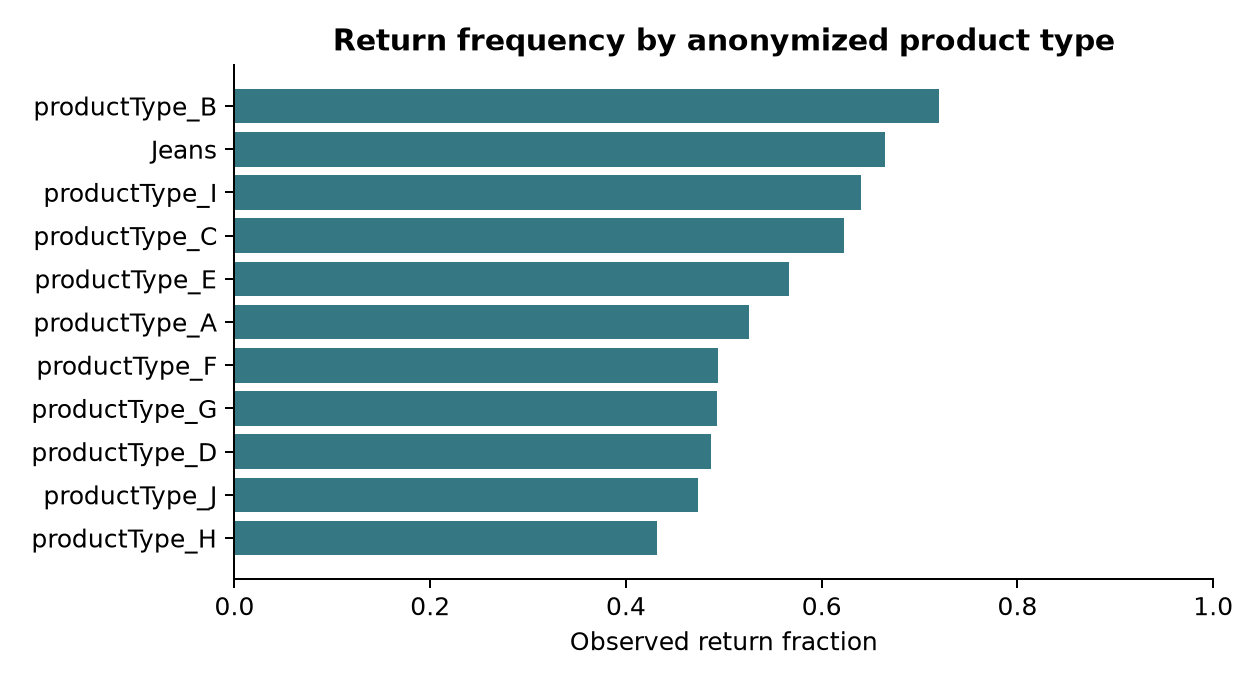
\includegraphics[width=.49\linewidth]{product_return_rates.png}\hfill
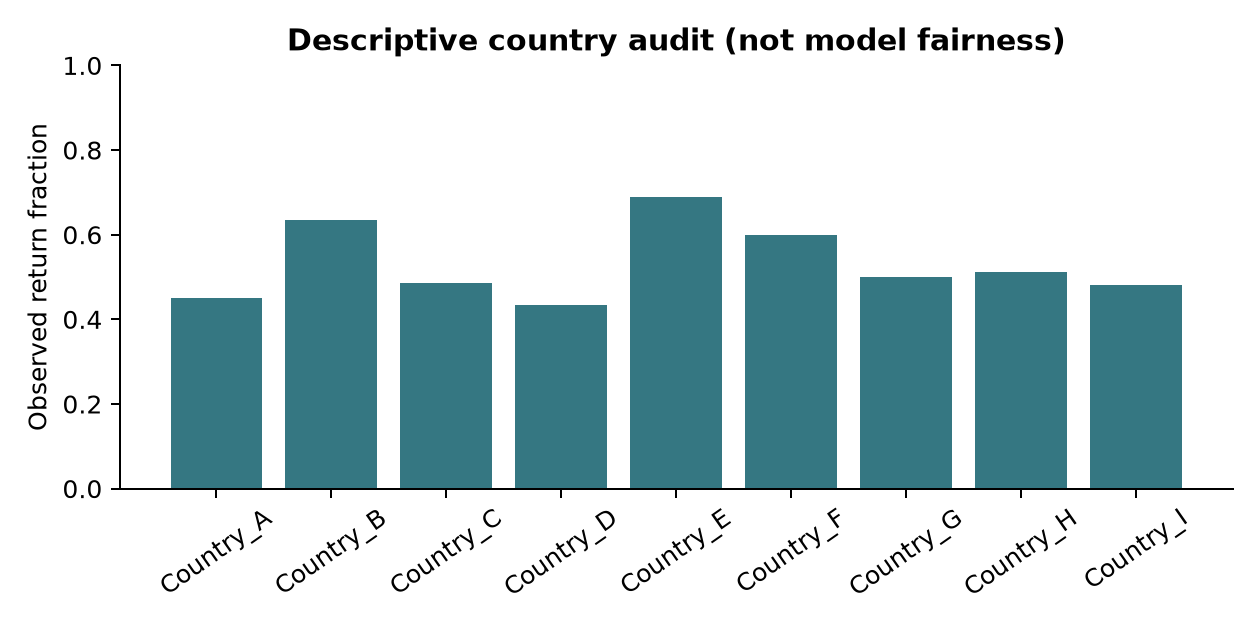
\includegraphics[width=.49\linewidth]{country_audit.png}
\caption{Return rate by product type (left) ranges from 43\% to 72\%. Return rate by anonymised shipping country (right) ranges from 43\% to 69\%, and Country\_G holds over half of the sample.}
\label{fig:eda}
\end{figure}

\section{Features and validation strategy}\label{sec:features}
\begin{table}[H]\centering\small
\begin{tabularx}{\linewidth}{p{.30\linewidth}p{.17\linewidth}X}
\toprule Field & Final model & Reason\\ \midrule
Product type, brand & Used & Product attributes known at order time. One-hot encoded.\\
Shipping country & Used & Known at checkout. One-hot encoded.\\
Customer age, gender, premier membership & Used & Stored on the customer account. Median-imputed and scaled.\\
Average price and discount & Excluded & Product averages over a period that may include the purchase itself.\\
Return counts, rates and reasons & Excluded & Computed from outcomes, including the one being predicted.\\
Customer and variant IDs & Excluded & Used only to join tables and split customers.\\ \bottomrule
\end{tabularx}
\caption{Input choices. Every used input is available when the order is placed.}
\end{table}

A seeded customer split held out 30\% of customers and divided them equally into validation and test sets, so no customer appears in more than one partition. Preprocessing and models were fitted on training data, validation chose models and cutoffs, and the test set was used only for the final results.

\begin{table}[H]\centering
\begin{tabularx}{.8\linewidth}{Xrrrr}
\toprule Partition & Purchases & Customers & Returned & Kept\\ \midrule
Train & 69,996 & 66,139 & 38,150 & 31,846\\
Validation & 14,964 & 14,173 & 8,102 & 6,862\\
Test & 15,040 & 14,173 & 8,232 & 6,808\\ \bottomrule
\end{tabularx}
\caption{Customer-separated partitions with zero customer overlap.}
\end{table}

\section{Models}
\subsection{Baselines and the Deliverable 2 model}
The majority baseline predicts a return for every purchase. The product-type rule predicts the training return rate of the purchase's product type and flags it at 0.50. In Deliverable~2 we compared logistic regression (\(C \in \{0.1, 1, 10\}\)) and decision trees on product type and brand. Logistic regression with \(C=0.1\) won (validation ROC-AUC 0.616). Its cutoff was chosen by maximising validation F1. Because 55\% of purchases are returns, predicting ``returned'' for everything already gives F1 = 0.707, so the search settled on 0.42 and the model flagged every test purchase.

\subsection{Final model}
\begin{center}
\stage{Six order-time\\inputs}\(\,\to\,\)\stage{Impute, one-hot\\encode and scale}\(\,\to\,\)\stage{Histogram\\gradient boosting}\(\,\to\,\)\stage{Probability and\\0.57 cutoff}
\end{center}
{\small\textbf{Model pipeline.} The fitted preprocessing and classifier are saved as one scikit-learn~\cite{sklearn} pipeline, together with the cutoff and the input options used by the app.}

Gradient boosting builds an ensemble of shallow regression trees, each fitted to the gradient of the log loss left by the trees before it~\cite{friedman}. The histogram variant bins inputs before searching for splits, which makes training fast~\cite{lightgbm}. We compared logistic regression and boosting on both the Deliverable~2 inputs and the six order-time inputs. Only order-time candidates could be selected.

\begin{table}[H]\centering\small
\begin{tabularx}{\linewidth}{Xlrr}
\toprule Model & Settings & Two inputs & Six inputs\\ \midrule
Logistic regression & \(C=0.1\) & 0.6156 & 0.6492\\
Logistic regression & \(C=1\) or \(10\) & 0.6156 & 0.6492\\
Gradient boosting & depth 3, rate 0.03 & 0.6168 & 0.6522\\
Gradient boosting & depth 3, rate 0.10 & 0.6151 & 0.6513\\
Gradient boosting & depth 5, rate 0.03 & 0.6151 & \textbf{0.6527}\\
Gradient boosting & depth 5, rate 0.10 & 0.6151 & 0.6497\\ \bottomrule
\end{tabularx}
\caption{Validation ROC-AUC. Boosting models use 300 iterations. Adding the order-time inputs improved every model by about 0.035, more than the choice between model families.}
\end{table}

The winner was gradient boosting with depth 5 and learning rate 0.03. We then searched cutoffs from 0.30 to 0.70 for the highest validation balanced accuracy, the mean of the recall on returns and the recall on kept purchases. Unlike F1, this metric gives no credit to flagging everything. The chosen cutoff is 0.57, with validation balanced accuracy 0.620.

\begin{figure}[H]\centering
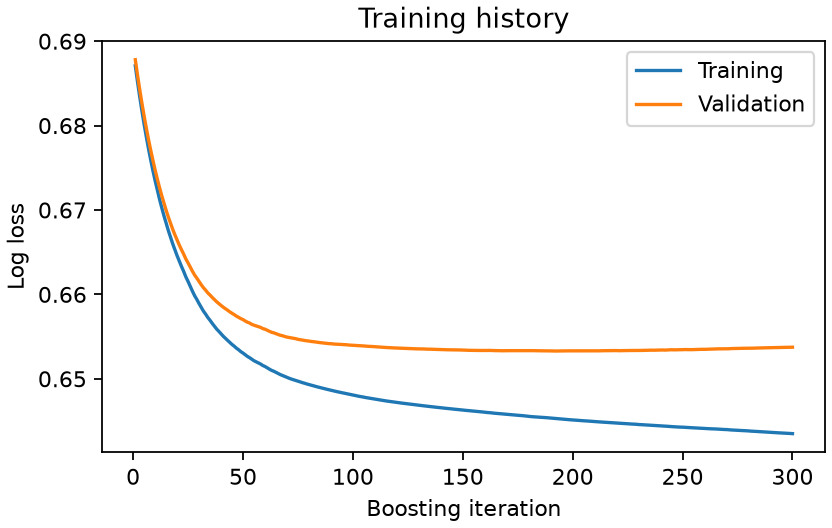
\includegraphics[width=.49\linewidth]{final_training_history.png}\hfill
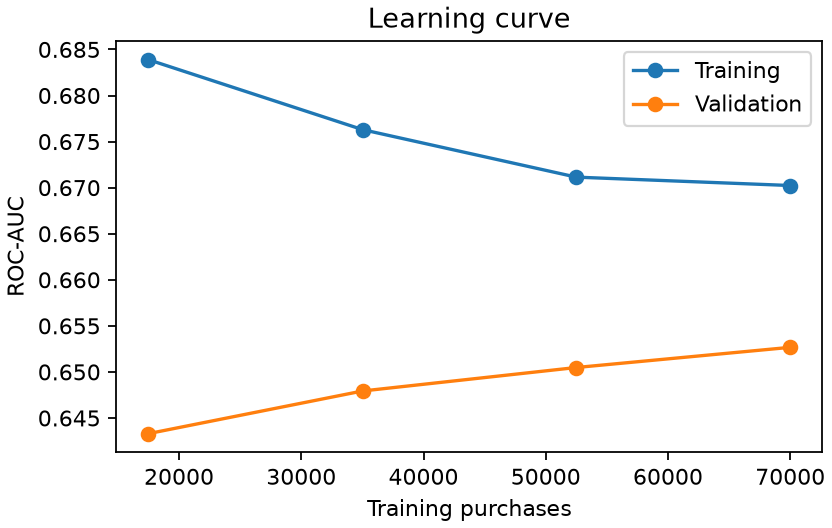
\includegraphics[width=.49\linewidth]{final_learning_curve.png}
\caption{Training history (left): validation log loss levels off after about 150 boosting iterations while training loss keeps falling slowly, so 300 iterations overfit only slightly. Learning curve (right): validation ROC-AUC still rises with more training purchases, so more data would likely help.}
\end{figure}

\section{Results}
All results in this section come from the 15,040 test purchases, which no model saw during training or selection.

\begin{table}[H]\centering
\begin{tabularx}{\linewidth}{Xrrrrr}
\toprule Method & Accuracy & Precision & Recall & F1 & ROC-AUC\\ \midrule
Majority baseline & 0.547 & 0.547 & 1.000 & 0.707 & 0.500\\
Product-type rule & 0.580 & 0.666 & 0.466 & 0.548 & 0.607\\
Deliverable 2 logistic model & 0.547 & 0.547 & 1.000 & 0.707 & 0.614\\
\textbf{Final gradient boosting model} & \textbf{0.607} & \textbf{0.678} & 0.536 & 0.599 & \textbf{0.651}\\ \bottomrule
\end{tabularx}
\caption{Held-out results. ROC-AUC measures ranking across all cutoffs. Precision is the share of flagged purchases that were returned. Recall is the share of returns that were flagged.}
\end{table}

The final model has the best accuracy, precision and ROC-AUC. Its F1 is lower than the majority baseline only because that baseline has perfect recall by flagging everything. Compared with the product-type rule, the final model catches 581 more returns (4,414 against 3,833) for 175 more false alarms (2,099 against 1,924).

\begin{figure}[H]\centering
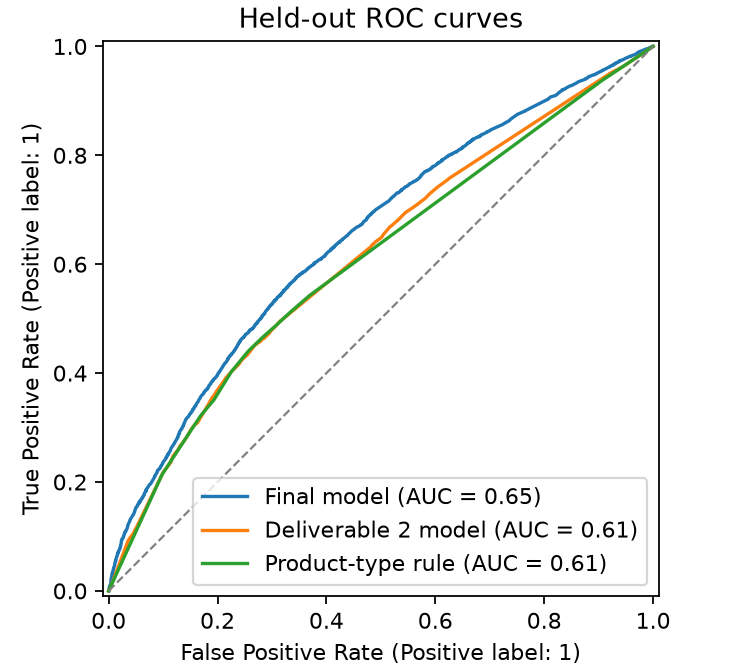
\includegraphics[width=.47\linewidth]{final_roc_curve.png}\hfill
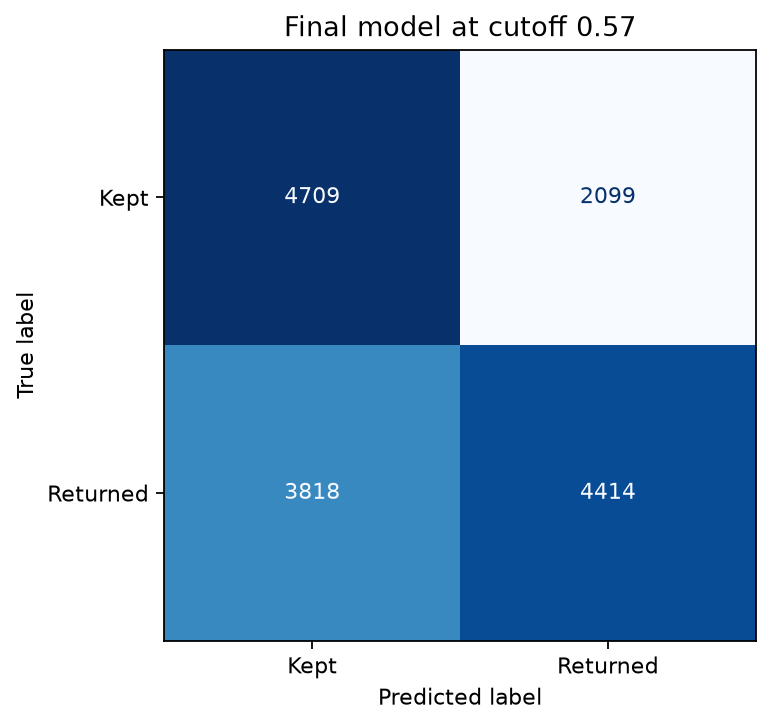
\includegraphics[width=.45\linewidth]{final_confusion_matrix.png}
\caption{Left: the final model's ROC curve lies above both earlier methods at almost every false-positive rate. Right: at the 0.57 cutoff the model flags 6,513 purchases, of which 4,414 were returned.}
\end{figure}

\begin{table}[H]\centering\small
\begin{tabularx}{\linewidth}{llllrrll}
\toprule Product & Brand & Country & Age & Male & Premier & Probability & Actual\\ \midrule
productType\_B & Brand\_K & Country\_E & 73 & 0 & 0 & 0.924 & Returned\\
productType\_B & Brand\_K & Country\_E & 28 & 0 & 0 & 0.873 & Kept\\
productType\_B & Brand\_K & Country\_E & 71 & 0 & 0 & 0.872 & Returned\\
productType\_H & Pull\&Bear & Country\_D & 20 & 1 & 0 & 0.220 & Kept\\
productType\_H & Pull\&Bear & Country\_G & 19 & 0 & 0 & 0.217 & Kept\\
productType\_H & Pull\&Bear & Country\_G & 19 & 1 & 0 & 0.211 & Returned\\ \bottomrule
\end{tabularx}
\caption{Sample predictions: the three highest and three lowest scores among distinct held-out purchases. Two of the six are errors, which shows that even confident scores can be wrong.}
\end{table}

\section{Error analysis and bias check}
Table~\ref{tab:groups} shows how errors fall across shipping countries and the largest product types. Country\_E and productType\_B have high training return rates, and the model flags almost every purchase in them. Country\_G and productType\_J have lower rates, and the model misses most of their returns. The model has therefore learned mostly group-level return rates. Within a group it separates returns from kept purchases only weakly, so it over-flags in high-return groups and under-flags in low-return groups.

\begin{table}[H]\centering\small
\begin{tabularx}{\linewidth}{Xrrrrr}
\toprule Group & Purchases & Returned & Recall & False-positive rate & Missed returns\\ \midrule
Country\_E & 3,553 & 2,446 & 0.952 & 0.894 & 117\\
Country\_G & 8,334 & 4,189 & 0.356 & 0.184 & 2,699\\
Country\_H & 1,131 & 587 & 0.394 & 0.200 & 356\\
Country\_D & 667 & 308 & 0.221 & 0.103 & 240\\ \midrule
productType\_B & 2,427 & 1,759 & 0.982 & 0.979 & 32\\
Jeans & 1,367 & 887 & 0.900 & 0.835 & 89\\
productType\_J & 6,908 & 3,251 & 0.279 & 0.148 & 2,344\\
productType\_H & 1,152 & 514 & 0.253 & 0.119 & 384\\ \bottomrule
\end{tabularx}
\caption{Held-out errors for the four largest countries and four selected product types. Every group listed has at least 20 returned and 20 kept purchases. Full results are in \texttt{reports/evidence/final\_errors.json}.}
\label{tab:groups}
\end{table}

\textbf{Why samples fail.} The inputs describe the product category and the customer in broad terms. They say nothing about size, fit, colour, the exact price paid or the customer's past returns, which are the usual reasons for fashion returns. Two purchases with the same inputs receive the same score even when one is returned and the other is kept, as the second row of the sample table shows.

\textbf{Fairness.} The large differences in false-positive rate between countries mean that customers in some countries would be flagged far more often. Because country labels are anonymised, we cannot tell which real regions are affected. Gender is an input. It is known at order time, but using it for decisions about individual customers would raise fairness concerns. For these reasons the application presents scores as a planning signal, and its About page states these limits.

\section{Deployed application}
\begin{center}
\stage{Streamlit\\interface}\(\,\to\,\)\stage{\texttt{predict.py}\\checks inputs}\(\,\to\,\)\stage{Saved pipeline\\(joblib)}\(\,\to\,\)\stage{Probability, band\\and explanation}
\end{center}
{\small\textbf{Application architecture.} The interface and the backend run in one Python process, and the model is loaded once and cached.}

The application is written in Streamlit~\cite{streamlit} and hosted on Streamlit Community Cloud from the GitHub repository. It has three tabs.

\begin{itemize}
\item \textbf{Single purchase.} Drop-down lists offer only the product types, brands and countries the model was trained on, so users cannot enter unknown values. The score updates as soon as an input changes. The app shows the return probability, a likely-return or likely-keep decision, a risk band and the product type's training return rate for context.
\item \textbf{Explanation.} For each input, the app swaps in the most common training value and reports how much the probability changes. This model-agnostic check tells the user which inputs push this purchase's risk up or down.
\item \textbf{Upload a file.} Users upload a CSV of purchases and receive a scored table they can download. The backend reports missing columns as errors. Unknown categories, invalid ages and invalid flags become warnings, and those values are treated as unknown instead of stopping the whole file. A sample file of 25 held-out purchases is provided for demonstrations.
\item \textbf{About.} A summary of the data, model, cutoff, held-out results and limitations.
\end{itemize}

The file \texttt{tests/test\_predict.py} holds eight automated tests for the backend module \texttt{src/predict.py}. They check the saved model, single and batch scoring, missing columns, empty files, invalid values, the explanation and the risk bands.

\begin{figure}[H]\centering
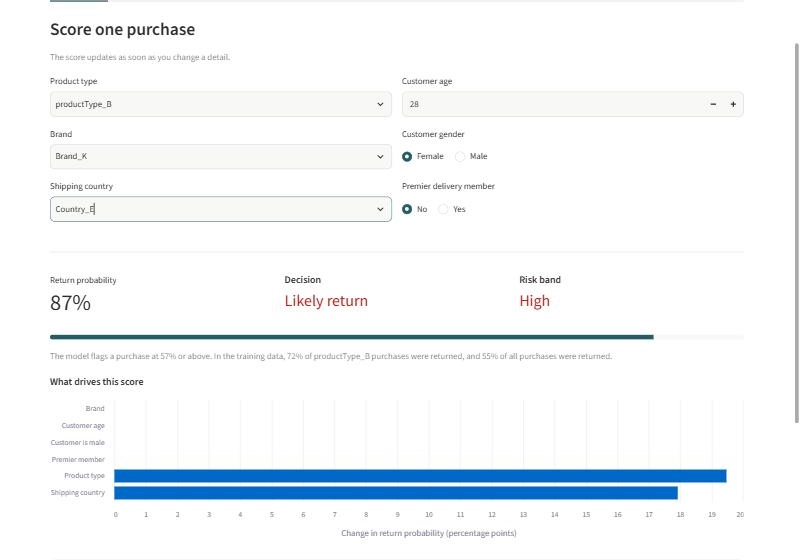
\includegraphics[width=.49\linewidth]{app_single.png}\hfill
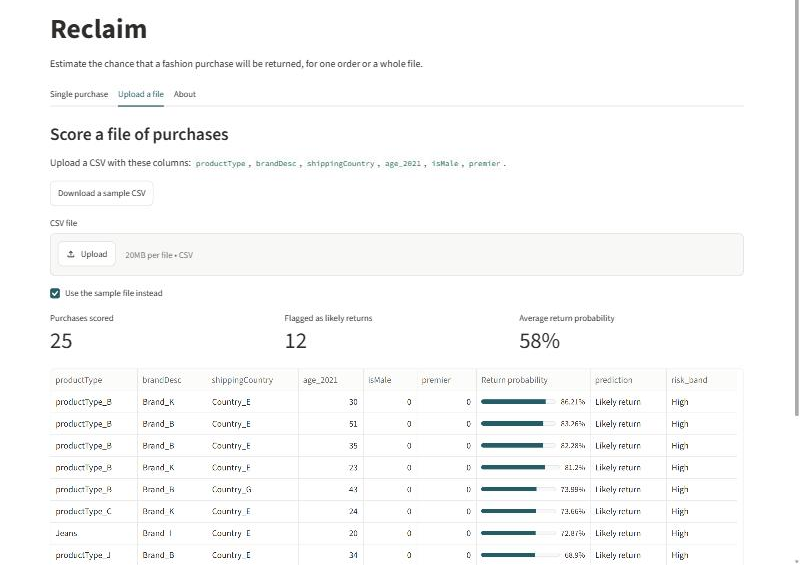
\includegraphics[width=.49\linewidth]{app_upload.png}
\caption{The hosted application. Left: scoring a single purchase, with its explanation. Right: scoring the sample CSV file.}
\end{figure}

\section{Limitations and future work}
\begin{itemize}
\item \textbf{Modest signal.} A ROC-AUC of 0.651 is clearly better than chance and than the baselines, but the model still misclassifies about 39\% of purchases.
\item \textbf{Population.} The source selected customers with a return history, so probabilities are higher than for a typical shopper. Excluded events, about 38\% of the original data, had a slightly higher return rate.
\item \textbf{Time.} All partitions come from one training period. The official later-period test release was not used, so we have not measured how the model holds up over time.
\item \textbf{Anonymised labels.} Most category names are codes, which limits interpretation and makes the app less friendly for real users.
\item \textbf{Future work.} Evaluate on the later-period release; add customer history built only from earlier purchases; add exact order prices if timestamps become available; calibrate the probabilities; and set the cutoff from real costs of missed returns and false alarms.
\end{itemize}

\section{Contributions}
\begin{table}[H]\centering\small
\begin{tabularx}{\linewidth}{@{}llX@{}}
\toprule Deliverable & GitHub author & Work\\ \midrule
1 & Mahad-Jawad & Acquisition, provenance, checksum verification and cleaning\\
1 & taimurrrr & Preprocessing, exploratory charts and pipeline validation\\
1 & Soban06 & Problem definition, report and integration\\ \midrule
2 & Mahad-Jawad & Input checks, customer split and split evidence (\commit{c95f764}, \commit{3973a72}, \commit{54510e3})\\
2 & taimurrrr & Baselines, model selection and learning curves (\commit{1cf72ca}, \commit{deca2be})\\
2 & Soban06 & Held-out evaluation, group checks and confusion matrix (\commit{fd8d720}, \commit{63d1435})\\ \midrule
3 & taimurrrr & Final model training, cutoff selection, training history and learning curve (\commit{4ee45f8}, \commit{f8985a6})\\
3 & Mahad-Jawad & Prediction backend, held-out evaluation and tests (\commit{4488d62}, \commit{d716bf1}, \commit{2b9b00f})\\
3 & Soban06 & Streamlit application, deployment, README and final report (\commit{c88d992}, \commit{ebc9591})\\ \bottomrule
\end{tabularx}
\end{table}
AI assistance was used to generate code and draft documentation. Each member reviewed, ran and committed their own part, as recorded in the repository history.

\section*{Reproducibility}
The README lists the commands that rebuild the data, models, figures and evidence from the original source. Package versions are pinned in \texttt{requirements-lock.txt}. All metrics in this report are stored as JSON files in \texttt{reports/evidence/}.

\small
\begin{thebibliography}{9}
\bibitem{data} ASOS. \emph{ASOS GraphReturns dataset}. Open Science Framework, 2022. \url{https://osf.io/c793h/}. CC BY 4.0.
\bibitem{paper} J. McGowan et al. \emph{A Dataset for Learning Graph Representations to Predict Customer Returns in Fashion Retail}. arXiv:2302.14096, 2023. \url{https://arxiv.org/abs/2302.14096}.
\bibitem{friedman} J. H. Friedman. Greedy function approximation: a gradient boosting machine. \emph{Annals of Statistics}, 29(5):1189--1232, 2001.
\bibitem{lightgbm} G. Ke, Q. Meng, T. Finley, T. Wang, W. Chen, W. Ma, Q. Ye and T.-Y. Liu. LightGBM: a highly efficient gradient boosting decision tree. In \emph{Advances in Neural Information Processing Systems 30}, 2017.
\bibitem{sklearn} F. Pedregosa et al. Scikit-learn: machine learning in Python. \emph{Journal of Machine Learning Research}, 12:2825--2830, 2011.
\bibitem{streamlit} Streamlit. \emph{Streamlit documentation}. \url{https://docs.streamlit.io/}. Accessed November 2026.
\end{thebibliography}
\end{document}
